\documentclass{llncs}
\usepackage{algorithm,algorithmic}
\usepackage{graphicx}
\usepackage{placeins}
\usepackage{float}
\usepackage{subfigure}
\usepackage{multirow}    
\usepackage{llncsdoc}
\begin{document}
\markboth{\$ Simulator for Distributed Sleepy 
Consensus}{\$ Simulator for Distributed Sleepy Consensus}
\thispagestyle{empty}
\begin{flushleft}
\LARGE\bfseries Distributed Consensus\\[2cm]
\end{flushleft}
\rule{\textwidth}{1pt}
\vspace{2pt}
\begin{flushright}
\Huge
\begin{tabular}{@{}l}
Simulator for\\
Sleepy Consensus Protocol\\[6pt]
{\Large SJTU 2017 Cornell Summer Workshop}
\end{tabular}
\end{flushright}
\rule{\textwidth}{1pt}
\vfill
\begin{flushleft}
\large\itshape
\begin{tabular}{@{}l}
{\Large\upshape\bfseries Instructor }\\[8pt]
Elaine\enspace Shi \\[5pt]
Cornell\enspace University\\[5pt]
\end{tabular}
\end{flushleft}
\newpage
%
\section*{Our Group:}
%
\begin{flushleft}
\begin{tabular}{l@{\quad}l@{\hspace{3mm}}l@{\qquad}l}
$\bullet$&\multicolumn{3}{@{}l}{\bfseries Framework Team Members}\\[1mm]
% &\multicolumn{3}{@{}l}{Springer-Verlag}\\
% &\multicolumn{3}{@{}l}{Computer Science Editorial}\\
% &\multicolumn{3}{@{}l}{Tiergartenstra�e 17}\\
% &\multicolumn{3}{@{}l}{69121 Heidelberg}\\
% &\multicolumn{3}{@{}l}{Germany}\\[0.5mm]
 & Junxiang Huang       & & 841450297@qq.com\\
 & Yifei Pu       & &pkq2006@gmail.com\\[2mm]
$\bullet$&\multicolumn{3}{@{}l}{\bfseries Honest Node Team Members}\\[1mm]
 & Tiancheng Xie       & & wjxtcsgx@hotmail.com\\
 & Jiaheng Zhang      & &ZHANGJIAHENG@sjtu.edu.cn\\
 & Xiaotian You    &  & youxiaotian@hotmail.com\\
 & Shuyang Tang         &  & tangshuyang25@163.com\\
 & Chengyao Li   &  & cyli2014@sjtu.edu.cn\\[2mm]
 $\bullet$&\multicolumn{3}{@{}l}{\bfseries Adversary Members}\\[1mm]
 & Qingrong Chen      & & chenqingrong@sjtu.edu.cn\\
 & Ruisheng Cao      & &211314@sjtu.edu.cn\\
 & Shiquan Zhang    &  & zsq007@sjtu.edu.cn\\
 & Haochen Huang  &  & hhc98598@189.cn\\[2mm]
$\bullet$&\multicolumn{3}{@{}l}{\bfseries Integrators}\\[1mm]
 & Feiyang Qiu   &  & st.yeah@gmail.com\\
 & Lingkun Kong  &  & klk316980786@sjtu.edu.cn\\
 & Lanqing Liu    &  & sunnysunny@sjtu.edu.cn\\
 & Jialu Li          &  & 790359064@qq.com\\[2mm]
\\
\\
\\
\\
\\
\\
\\
% \noalign{\rule{\textwidth}{1pt}}
% \noalign{\vskip2mm}
$\bullet$&\multicolumn{3}{@{}l}{\bfseries Where to find our project?}\\[1mm]
 & https://github.com/initc3/sleepysim & & SleepySim\\[2mm]
\end{tabular}
\end{flushleft}


%
\newpage
\tableofcontents
\newpage
%
\section{Introduction}
\quad Consensus protocol serves as the core of distributed computing and also provides a foundational building block for cryptocurrency protocols. In traditional cryptocurrency schemes, proof-of-work (PoW) is leveraged to provide consistency and chain quality for the underlying blockchain. However, proof-of-work is notoriously indifferent for its waste of energy and the potential of the computing power centralization. To face this issue, proof-of-stake (PoS) is proposed to replace proof-of-work. In  Pass and Shi's \emph{sleepy consensus} article (eprint 2016/918) \cite{Sleepy}, a PoS protocol is constructed to realize consensus on the “linearly ordered log” abstraction -- often referred to as state machine replication or linearizability in the distributed systems literature. This scheme is named as sleepy consensus protocol, which respects two important resiliency properties, i.e., consistency and liveness. Moreover, in sleepy consensus model, players can be either online (alert) or offline (asleep), and their online status may change at any point during the protocol execution.

Algorithm \ref{algo1} presents how sleepy consensus protocol works. The protocol takes a parameter $p$ as input, where $p$ denotes the probability each node is elected leader in a single time step. All nodes that just spawned will invoke the init entry point. During initialization, a node generates a signature key pair and registers the public key with the public-key infrastructure $F_{CA}$.
\vspace{-4mm}
\begin{algorithm}
\caption{Sleepy Consensus Protocol}
\label{algo1}
\footnotesize
  \begin{algorithmic}[1]
  \renewcommand{\algorithmicrequire}{\textbf{If On Initialization:}}
  \renewcommand{\algorithmicensure}{\textbf{If On Received \emph{chain'}:}}
  % \renewcommand{\algorithmiclastcon}{\textbf{Every Time Step:}}
  \REQUIRE 
  \STATE Let $(pk,sk):=\sum.\mbox{gen}()$
  \STATE Register $pk$ with $F_{CA}$
  \STATE Let \emph{chain} $:=$ \emph{genesis}
  
  \ENSURE  
  \STATE Assert $|$\emph{chain'}$| > |$\emph{chain}$|$ and \emph{chain'} is valid w.r.t. eligible and the current time $t$ 
  \STATE \emph{chain} $:=$ \emph{chain'} and gossip \emph{chain}

  \renewcommand{\algorithmicensure}{\textbf{Every Time Step:}}
  \ENSURE 
  \STATE Receive input $\mbox{transactions}(\mbox{txs})$
  \STATE Let $t$ be the current time
  \IF {$\mbox{eligible}^t(P)$ where $P$ is the current node's party identifier}
  \STATE Let $\sigma := \sum.\mbox{sign}(sk, \mbox{\emph{chain}}[−1].h, \mbox{txs}, t), h':= d(\mbox{\emph{chain}}[−1].h, \mbox{txs}, t, P, \sigma)$
  \STATE Let $B := (\mbox{\emph{chain}}[−1].h, \mbox{txs}, t, P, \sigma, h')$, let $\mbox{\emph{chain}} := \mbox{\emph{chain}}||B$ and gossip \emph{chain}
  \ENDIF
  \STATE Output $\mbox{\emph{extract}}(\mbox{\emph{chain}})$ to $Z$ where $\mbox{\emph{extract}}()$ is the function outputs an ordered list containing the $\mbox{txs}$ extracted from each block in \emph{chain}
  \renewcommand{\algorithmicensure}{\textbf{\emph{Subroutine} $\mbox{eligible}^t(P)$:}}
  \ENSURE 
  \IF {$H(P, t) < D_p$ and $P$ is a valid party of this protocol.} \RETURN 1
  \ELSE \RETURN 0
  \ENDIF
  \end{algorithmic}
\end{algorithm}
\vspace{-5mm}

Now, the sleepy protocol proceeds very much like a proof-of-work blockchain, except that instead of solving computational puzzles, in this protocol a node can extend the chain at time $t$ iff it is elected leader at time $t$. To extend the chain with a block, a leader of time $t$ simply signs a tuple containing the previous block’s hash, the node’s own party identifier, the current time $t$, as well as a set of transactions to be confirmed. Leader election can be achieved through a public hash function $H$ that is modeled as a random oracle.
The difficulty parameter $D_{p}$ is defined such that the hash outcome is less than $D_{p}$ with probability $p$. For simplicity, here we describe the scheme with a random oracle $H$ -- however as we explain in this section, $H$ can be removed and replaced with a pseurdorandom function and a common reference string.

In this document, we build a simulator for monitoring the real-world performance of sleepy consensus protocol by constructing a framework which implements Algorithm \ref{algo1}, as well as imitating behaviors of honest players and corrupted/adversarial players in the meanwhile. After analyzing the simulating results, \textbf{we know ... add text here}

This document is organized as follows. In Section 2, we introduce the framework of simulator. In Section 3, we present how honest players work while simulating. And in Section 4, we imitate the adversarial players' behavior and attack the sleepy consensus protocol by several algorithms. We give the analysis of simulating results in Section 5. Finally, we draw conclusions in Section 6.

\section{The Framework of Simulator}
%
In this section, we will illustrate the construction of the framework of our simulator, which includes \textbf{add text here}

%
\subsection{Controller}
...

\section{The Imitation of Honest Players}
\subsection{Algorithm for Honest Players}
In our program, the honest nodes use the algorithm of sleepy consensus. To be specific,  	There are some steps for the algorithm.
\begin{itemize}
	\item First, the nodes will elect a leader using the hash function of identity and current time. If
		 $$H(identity, current time) < D$$,
		 where D denotes difficulty, then $Node[identity]$ will be elected to be a leader.\\
	\item Second, the leader can sign the block using the hash value of previous block, transactions and time, then broadcasts.
		 $$Block = sign(sk, block, Trans, time)$$
	\item When one honest node receive a new chain, if the time in block is strictly increasing and the time in the blocks is not in the future, it will update its chain with the new chain.	 
\end{itemize}
\subsection{The process to simulate sleepy consensus}
There are several steps to simulate the algorithm of sleepy consensus in our program.
\begin{itemize}
	\item First of all, in every round, the controller will 	let every node to run.\\ 
	\item Second, the honest node will ask network controller for messages.\\
	\item Third, the network controller will send related message to every node.\\ 
	\item Then every honest node will ask the controller whether it  has been elected a leader.\\
	\item Next, if one honest node is not elected to be a leader, it will do nothing. However, if it is a leader, it will sign one new block using its secret key with the hash value of previous block, transactions and time stamp. Then it will broadcast it.\\
	\item Finally, whatever one honest node has done, it will give some feedback to controller and network controller.\\
\end{itemize}
%
\section{The Imitation of Adversarial Players}
\quad The previous section introduces the implementation of the honest players' behavior under the sleepy consensus protocol in simulator. This section, in contrast, will present the imitatation of the adversarial players' behavior, which aims to hinder the normal functioning of sleepy consensus protocol under current framework structure. And we design four different attacking algorithms to try to break the consensus between different nodes, i.e., players in the distributed system. What should be noticed is that the adversaries cannot betray the rules established by the framework, while they can only control the network message transportation, i.e., intercepting and delaying the message from honest players. Also, an adversary can manipulate several corrupted nodes in the system, by which adversary impose damage to the system under sleepy consensus protocol.

To simulate the attacks, we assume there is an an adversary lurking within the  framework, who owns competence to intercept all messages coming from honest nodes and decide which to delay in the transportation. Also, the adversary is able to access useful information from these message to fork blocks right behind the private chain he captures. Based on above setting, we design four attacking methods for adversary to smash the consensus holded by system, which are illustrated in following subsections.
\subsection{Na{\"i}ve Adversary Attack}
\quad The \emph{Na{\"i}ve Adversary Attack} corresponds to an attacking method that is quite simple and easy to be came up with when knowing how the sleepy consensus protocol works. Figure \ref{naive} illustrates how na{\"i}ve adversaries to break the consistency of sleepy consensus. In this figure, when honest players add blocks to the main chain which they think is longest (that is the reason why there are several folks in Figure \ref{naive} -- blocks linked by dashed arrows), adversaries mine their own private chain and check whether the length of longest added blocks is larger than security parameter $T$ in every time step. If the longest chain added by honest nodes has length larger than $T$ yet smaller than the length of private chain mined by adversaries, the attacker can, just like the red arrow in Figure \ref{naive}, add their private chain to a specific block in public chain and thus damaging the consistency of sleepy consensus, since some blocks which are confirmed be fixed in main chain are replaced by blocks forged by adversaries.
\vspace{-4mm}
\begin{figure}
\centering
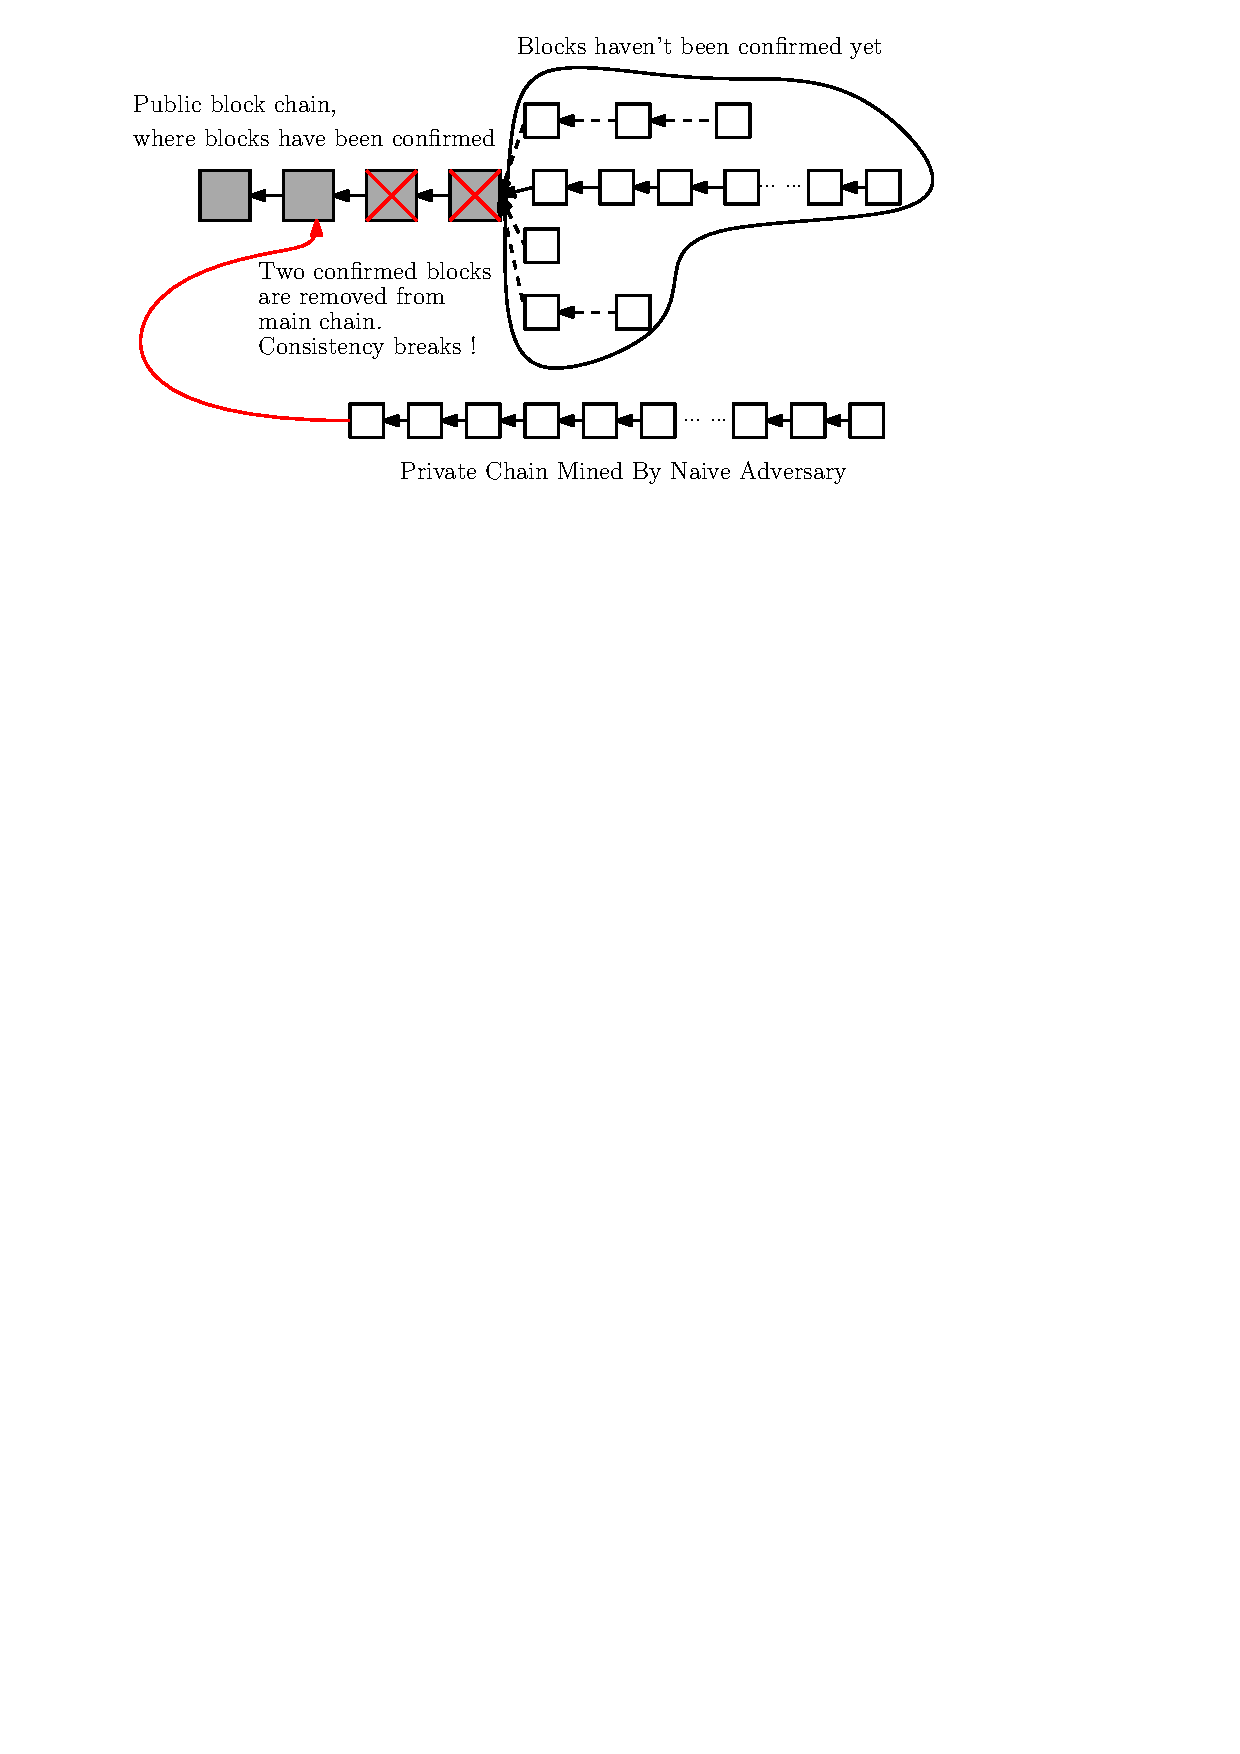
\includegraphics[width=4.3in]{Figures/Naive-Attack.pdf}
\vspace{-3mm}
\caption{This figure represents the attack which na{\"i}ve adversaries impose to the sleepy consensus. The consistency of consensus will break when the length of private chain mined by adversaries is larger than the length of the longest private chain mined by honest nodes, and the later one is supposed be larger than security parameter $T$, which denotes the time round number a block can be confirmed as secure, i.e., be eternally fixed in main block chain.}
\label{naive}
\end{figure}
\subsection{Selfish Adversary Attack}


\subsection{Stubborn Adversary Attack}

\subsection{Selfish Eclipse Attack}
%
\section{The Analysis of Simulating Results}
Here is the analysis of Simulating Results.
\section{Conclusion}
In conclusion....


\begin{thebibliography}{}  % (do not forget {})

\bibitem{Sleepy}
Pass, Rafael, and Elaine Shi. \emph{The sleepy model of consensus}. Cryptology ePrint Archive, Report 2016/918, 2016. http://eprint. iacr. org/2016/918, 2016.

\end{thebibliography}
%
\end{document}
